\section{Integrationstest}
\begin{tcolorbox}[title=Integrationstest]
    Im \textbf{Integrationstest} werden die \textbf{einzeln entwickelten und getesteten} Klassen, Module oder Komponenten zusammengeführt und ihr \textbf{korrektes Zusammenwirken} getestet:
    Im \textbf{Integrationstest} wird die korrekte Erfüllung des \textbf{Entwurfs} getestet.
\end{tcolorbox}

\subsection{Vorgehen}
Der \textbf{Integrationstest} hängt eng mit der Art der Integration zusammen, wobei sich die Typen der Integration nach der Art des Vorgehens (\textbf{Bottom-Up}, \textbf{Ad-hoc}, \textbf{Big-Bang}, \textbf{High-Frequency}) oder an der Architektur der Anwendung orientieren (\textbf{Bottom-up}, \textbf{Layer}, \textbf{Client/Server}).\\

\noindent
\textit{Wedemann} listet folgende Arten der Integration auf, wobei er sich u.a. auf \textit{Binder} (\cite{Bin99}), bezieht (vgl.~\cite[59]{Wed09c}):

\begin{itemize}
    \item \textbf{Bottom-Up-Integration}: Integration der Komponenten von den Blättern des Abhängigkeitsbaumes zur Wurzel
    \item \textbf{Layer-Integration}: Einteilung des Systems in verschiedene Schichten, die Bottom-Up oder Top-Down integriert werden (vgl.~\cite[688]{Bin99})
    \item \textbf{Client-Server-Integration}: Client- und Serverkomponenten werden schrittweise integriert
    \item \textbf{Ad-hoc-Integration}: Bauteile werden in der Reihenfolge ihrer Fertigstellung integriert
    \item \textbf{Big-Bang-Integration}: Alle Komponenten werden zusammengeführt und auf einmal getestet
    \item \textbf{High-Frequency-Integration}: Häufige und regelmäßige Wiederholung der Integration und der Integrationstests, bspw. beim \textit{push} in das Repository
\end{itemize}

\subsubsection*{Einsatz}
Der \textbf{Big-Bang-Ansatz} bedeutet geringen Erfolg und hohen Aufwand im Fehlerfall, was sich auf die meist unübersichtlichen Querwirkungen zurückführen läßt, die bei einem großen System mit vielen verschiedenen Komponenten und Klassen entstehen, die auf einen Schlag zusammengeführt werden.\\
Durchgesetzt hat sich vor allem die \textbf{Bottom-Up-Integration} bei gleichzeitiger \textbf{High-Frequency-Integration}. \textbf{Layer-} und \textbf{Client-Server-Integration} sind als Spezialfälle des \textbf{Bottom-Up-Ansatzes} einzuordnen

\subsubsection*{Bottom-Up}
Der \textbf{Bottom-Up-Ansatz} ist das normale Vorgehen beim Integrationstest (vgl.~\cite[60]{Wed09c}).\\
Hierbei werden die Klassen vorher einzeln im Klassentest getestet, danach im Integrationstest schrittweise zusammengeführt und ihre Zusammenarbeit getestet.
Abhängigkeiten werden durch von den entsprechenden Klassen abgeleitete \textbf{Mock-Objekte} simuliert.
In Abbildung~\ref{fig:bottomup} wird im \textbf{Klassentest} für \code{B} ein Mock für \code{C} erstellt, für \code{A} ein Mock für \code {B}.\\
Bei der Integration wird dann im ersten Schritt \code{B} und \code{C} integriert, im Erfolgsfall dann \code{A} und \code{B} und \code{C}.

\begin{figure}
    \centering
    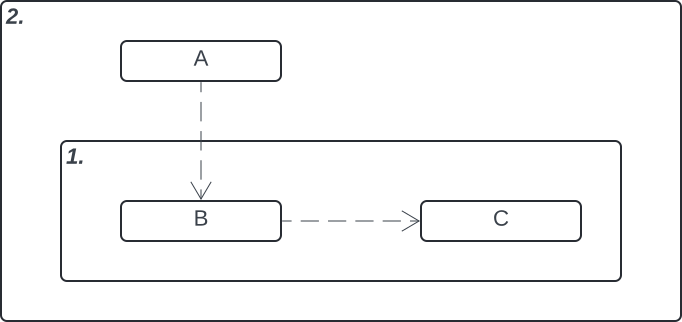
\includegraphics[scale=0.4]{part four/Testende Verfahren/img/bottomup}
    \caption{Beispiel für das Vorgehen bei der \textbf{Bottom-Up-Integration}. In Beispiel sind explizit UML-Abhängigkeiten notiert. (Quelle: in Anlehnung an \cite[Abb. 5.5, 60]{Wed09c})}
    \label{fig:bottomup}
\end{figure}

\subsubsection*{Alternative Vorgehensweisen}
Der \textbf{Bottom-Up-Ansatz} hat den Vorteil, dass die Klassen vor der Integration bereits im \textbf{Klassentest} getestet worden sind.
Fehler sind dann eher im Zusammenspiel der Klassen zu suchen und weniger in den Klassen selber.\\
Vor allem sind durch das schrittweise Vorgehen Defekte leichter zu lokalisieren.\\
Es entstehen allerdings viele Mock-Objekte, was mit einem hohen Aufwand verbunden ist.\\
Manchmal wird deshalb auf den Klassentest verzichtet und explizit von dem untersten Blatt des Abhängigkeitsbaumes bis zur Wurzel getestet, was den Nachteil hat, dass lange Ketten von Tests entstehen, die voneinander abhängig sind.
Auch die Aufteilung der Arbeit auf mehrere Entwickler erweist sich als schwierig.\\
In diesem Fall empfiehlt sich die Unterbrechung der Abhängigkeitskette durch Mock-Objekte, was bspw. auch bei Client-Server-Architekturen gemacht wird, bei denen die Endpoints eines Backend-Services durch Mock-Objekte simuliert werden.

\subsection{Integration von objektorientierten Systemen}
Bei Systemen, die mit objektorientierten Mitteln realisiert werden, ist durch \textbf{Vererbung} und \textbf{dynamische Bindung} zur Compile-Zeit nicht klar, welchen Typ zusammenarbeitende Instanzen besitzen.\\
Entsprechend müssten \textbf{alle möglichen Kombinationen} von Instanzen für einen \textbf{vollständigen} Test getestet werden.\\
In dem in Abbildung~\ref{fig:integration-vererbung} gezeigten Beispiel müsste also ein Test für \code{new A(new B())} und \code{new A(new B1())} existieren.

\begin{figure}
    \centering
    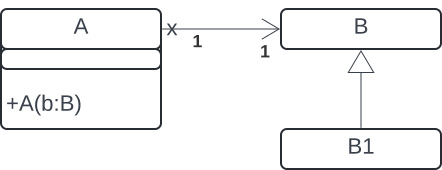
\includegraphics[scale=0.4]{part four/Testende Verfahren/img/integration-vererbung}
    \caption{Beispiel für Integration bei Vererbung. (Quelle: in Anlehnung an \cite[Abb. 5.6, 61]{Wed09c})}
    \label{fig:integration-vererbung}
\end{figure}

\noindent
Bei \textbf{großen Vererbungshierarchien} wächst die Anzahl der möglichen Kombinationen schnell an, weshalb eine durchdachte Automatisierung der Tests notwendig ist und evtl. geprüft werden muss, ob wirklich alle möglichen Paare getestet werden können (vgl.~\cite[61]{Wed09c}).

\subsubsection*{Test von Frameworks und Bibliotheken}
Schwieriger wird es beim Test von Bibliotheken oder Frameworks, die durch das Einfügen abgeleiteter Klassen benutzt werden, oder wenn Klassen durch Plugin-Schnittstellen zur Laufzeit hinzugefügt werden können: In diesem Fall ist ein vollständiger Test überhaupt nicht möglich.\\
In diesem Fall sind für den Test der Bibliothek bzw. des Frameworks die Klassen selber als \textbf{Inputdaten} zu betrachten: Die Entwickler müssen dann mit eigens dafür konstruierten Klassen das korrekte Verhalten in Grenzsituationen erproben (vgl.~\cite[62]{Wed09c}).